\documentclass[a4paper,11pt]{jsarticle}


% 数式
\usepackage{amsmath,amsfonts}
\usepackage{bm}
\usepackage{siunitx}
% 画像
\usepackage[dvipdfmx]{graphicx}
\usepackage{booktabs}


\begin{document}

\title{}
\author{}
\date{\today}


\section{図に示す容量型変圧器において、電圧計のインピーダンスの影響を除くための条件を求めなさい。}
\begin{figure}[htbp]
  \centering
  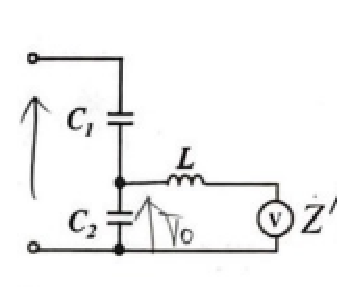
\includegraphics[width=5cm]{fig5.eps}
  \caption{}\label{fig1}
\end{figure}

図\ref{fig1}より、分圧の法則から、全体の電圧を$\dot{V_{1}}$、$C_{2}$にかかる電圧を$\dot{V_{0}}$、$Z$にかかる電圧を$\dot{V_{2}}$とすると、

\begin{align}
  \begin{split}
    \frac{\dot{V_{1}}}{\dot{V_{2}}}=\frac{\dot{V_{1}}}{\dot{V_{0}}}\cdot \frac{\dot{V_{0}}}{\dot{V_{2}}}
    \label{eq1}
  \end{split}
\end{align}

ここで、
\begin{align}
  \begin{split}
    \frac{\dot{V_{1}}}{\dot{V_{0}}}
    &=\frac{\frac{1}{j\omega C_{1}}+\frac{\frac{Z+j\omega L}{j\omega C_{2}}}{\frac{1}{j\omega C_{2}}+j\omega L+Z}}{\frac{\frac{Z+j\omega L}{j\omega C_{2}}}{\frac{1}{j\omega C_{2}}+j\omega L+Z}}\\
    &=\frac{\frac{\frac{1}{j\omega C_{2}}+j\omega L+Z}{j\omega C_{1}}+\frac{Z+j\omega L}{j\omega C_{2}}}{\frac{Z+j\omega L}{j\omega C_{2}}}\\
    &=\frac{\frac{1}{j\omega }+j\omega C_{2}L+ZC_{2}+ZC_{1}+j\omega LC_{1}}{C_{1}(Z+j\omega L)}\\
    &=\frac{(C_{1}+C_{2})(Z+j\omega L)+\frac{1}{j\omega }}{C_{1}(Z+j\omega L)}\\
    &=\frac{C_{1}+C_{2}}{C_{1}}+\frac{\frac{1}{j\omega }}{C_{1}(Z+j\omega L)}
    \label{eq2}
  \end{split}
\end{align}

また、
\begin{align}
  \begin{split}
    \frac{\dot{V_{0}}}{\dot{V_{2}}}
    &=\frac{j\omega L+Z}{Z}
    \label{eq3}
  \end{split}
\end{align}

となるから、式\eqref{eq1}$\sim $\eqref{eq3}より、

\begin{align}
  \begin{split}
    \frac{\dot{V_{1}}}{\dot{V_{2}}}
    &=\left(\frac{C_{1}+C_{2}}{C_{1}}+\frac{1}{j\omega C_{1}(Z+j\omega L)}\right)\left(\frac{Z+j\omega L}{Z}\right)\\
    &=\frac{C_{1}+C_{2}}{C_{1}}\left(1+\frac{j\omega L}{Z}\right)+\frac{1}{j\omega C_{1}Z}\\
    &=\frac{C_{1}+C_{2}}{C_{1}}+\frac{C_{1}+C_{2}}{C_{1}}\frac{j\omega L}{Z}+\frac{1}{j\omega C_{1}Z}\\
    &=\frac{C_{1}+C_{2}}{C_{1}}+\frac{1-\omega ^{2}L(C_{1}+C_{2})}{j\omega C_{1}Z}
    \label{eq4}
  \end{split}
\end{align}

電圧計のインピーダンスの影響を除くためには、式\eqref{eq4}の右辺第二項が0となる必要があるため、

\begin{align}
  \begin{split}
    1-\omega ^{2}L(C_{1}+C_{2})
    &=0\\
    \omega ^{2}L(C_{1}+C_{2})
    &=1
    \label{eq5}
  \end{split}
\end{align}
の条件が必要となる。

\end{document}